\section{Transport Layer}
\subsection{Overview}
\begin{itemize}
    \item it is after the network layer $\rightarrow$ receiver transport layer communicates with the analogue sender transport layer
    \item it sends data of application layer $\rightarrow$ as fast as it decides\\$\rightarrow$ in order not to create congestions
    \item it is the last layer unpacked from the layers' stack\\$\rightarrow$ used to know how to send packets
\end{itemize}
There are 3 main types of protocols for transport layer:
\begin{itemize}
    \item UDP:
    \begin{itemize}
        \item[$\rightarrow$] it is light, fast, unreliable $\rightarrow$ used for streaming and online games
        \item[$\rightarrow$] it just forwards what it is received from application layer\\
        $\Rightarrow$ this implies:
        \begin{itemize}
            \item no ACK
            \item no congestion control
            \item no care about order in receiver
        \end{itemize}
    \end{itemize}
    \item TCP:
    \begin{itemize}
        \item[$\rightarrow$] it is reliable, end-to-end, two-way protocol $\rightarrow$ used for sending files
        \item[$\rightarrow$] it assures that receiver gets packets correctly and ordered $\rightarrow$ waiting for ACK
        \item[$\rightarrow$] there is control over flow and congestion $\rightarrow$ on receiver and on internet\\
        $\Rightarrow$ this implies:
        \begin{itemize}
            \item it cares about speed $\rightarrow$ not overwelming receiver
            \item it prevents bottleneck $\rightarrow$ it prevents packet-loss
            \item if packets aren't received correctly $\Rightarrow$ they won't go up in the layers' stack of receiver 
        \end{itemize}
        \item[$\rightarrow$] it is closed to IP $\rightarrow$ TCP/IP
        \item[$\rightarrow$] there are many protocols $\rightarrow$ new ones must be backwards-compatible
    \end{itemize}
    \item QUIC:
    \begin{itemize}
        \item[$\rightarrow$] it is faster and simpler than TCP $\Rightarrow$ no 3-way handshake, \dots
        \item[$\rightarrow$] transport $\Rightarrow$ UDP + new layer $\rightarrow$ to emulate only TCP good things
    \end{itemize}
\end{itemize}

Some definitions:
\begin{itemize}
    \item Capacity $\rightarrow$ total data transfer available
    \item Bandwidth $\rightarrow$ total data transfer available right now
    \item Throughput $\rightarrow$ what is sent out
    \item Goodput $\rightarrow$ what is received in
\end{itemize}

\subsection{TCP Protocol}
Characteristics:
\begin{itemize}
    \item it is byte-stream connection-oriented, reliable, full-duplex
    \item byte-stream:
    \begin{itemize}
        \item[$\rightarrow$] app writes bytes
        \item[$\rightarrow$] TCP sends segments $\Rightarrow$ $\approx 1.5$KB
        \item[$\rightarrow$] app reads bytes
    \end{itemize}
    \item it has flow and congestion control
    \item it is tied to the Internet Protocol (IP)
\end{itemize}

\subsubsection{TCP Reliability}
Characteristics:
\begin{itemize}
    \item it is used checksum $\rightarrow$ to detect bit level errors
    \item it is used sequence numbers $\rightarrow$ to detect sequencing errors
    $\Rightarrow$ so:
    \begin{itemize}
        \item[$\rightarrow$] duplicates packets are discarded
        \item[$\rightarrow$] packets can be reordered
        \item[$\rightarrow$] lost packets can be retransmitted
    \end{itemize}
    \item how to detect lost packets:
    \begin{itemize}
        \item[$\rightarrow$] Timeout-based Recovery:
        \begin{itemize}
            \item it requires sender to maintain data until it is ACKed
            \item based on RTT (Round Trip Time) $\rightarrow$ waiting before retransmitting
            \item it requires RTO (Retransmission TimeOut) calculation\\$\rightarrow$ accurate RTT estimators:
            \begin{itemize}
                \item low RTO $\rightarrow$ unneeded retransmissions
                \item high RTO $\rightarrow$ poor throughput
            \end{itemize}
            RTO $\Rightarrow$ it is about 4 times RTT
        \end{itemize}
        \item[$\rightarrow$] 3 Dupacks:
        \begin{itemize}
            \item Ack $\rightarrow$ packet received correctly, in order until packet $x$
            \item Dupack $\rightarrow$ same ack is received 2 times $\Rightarrow$ it happens:
            \begin{itemize}
                \item packet loss
                \item packet reordering
                \item AWND update
            \end{itemize}
            \item Problem $\rightarrow$ TCP timeouts lead to inactivity periods
            \item Proposal $\rightarrow$ use 3 duplicate ACKs to trigger retransmission
        \end{itemize}
    \end{itemize}
    \item Speed:\\[0.2cm]
    There are various types of icreasing speed $\rightarrow$ packets for RTT:
    \begin{itemize}
        \item[$\rightarrow$] linear (1-1, 2-2, 3-3, 4-4, \dots) $\rightarrow$ increase sliding windows (active packets)
        \item[$\rightarrow$] exponential (1-1, 2-2, 4-4, 8-8, \dots) $\rightarrow$ slide on every packet
        \item[$\rightarrow$] SSTHRESH $\rightarrow$ it doesn't start from first every retransmission:
        \begin{itemize}
            \item additive 
            \item multiplicative
        \end{itemize}
    \end{itemize}
    \item Flow Control:
    \begin{itemize}
        \item[$\rightarrow$] it blocks the sender from overwhelming the receiver
        \item[$\rightarrow$] Receiving side $\rightarrow$ AWND in returning ACKs is set by receiver\\
        $\Rightarrow$ how much space is left in its buffer
        \item[$\rightarrow$] Sending side $\rightarrow$ Sending Window represents the actual bytes sent out\\
        $SW = min(AW, CW)$ $\rightarrow$ min between advertised and congestion window
    \end{itemize}
    \item Congestion Control:
    \begin{itemize}
        \item[$\rightarrow$] Delay-Bandwitdth Product:
        \begin{itemize}
            \item delay $\rightarrow$ time passed from sender to receiver $\rightarrow$ known as ping
            \item bandwidth $\rightarrow$ how much is sent simultaneously on the channel
            \item RTT is twice the Delay
            \item bandwidth is distributed like:
            \begin{itemize}
                \item half the traffic is travelling
                \item half reached the receiver and is sending ACKs back
            \end{itemize}
        \end{itemize}
        \item[$\rightarrow$] it blocks the sender from overwhelming the network
        \item[$\rightarrow$] Idea:
        \begin{itemize}
            \item each source determines network capacity for itself
            \item it is used implicit feedback
        \end{itemize}
    \end{itemize}
    \item feedback algorithms are used for congestion control $\rightarrow$ AIMD
    \begin{itemize}
        \item[$\rightarrow$] Context:
        \begin{itemize}
            \item in the past people didn't think about wireless
            \item any loss in wired links $\Rightarrow$ caused by congestion (no error loss)\\
            $\rightarrow$ creation of algorithm to regulate this
        \end{itemize}
        \item[$\rightarrow$] AIMD (Additive Increase Multiplicative Decrease):
        \begin{itemize}
            \item adjust to changes in the available capacity
            \item CWND (Congestion Window):
            \begin{itemize}
                \item increase when congestion goes down
                \item decrease when congestion goes up
            \end{itemize}
            \item Congestion detection $\rightarrow$ assumption that lost packet $\Rightarrow$ congestion:
            \begin{itemize}
                \item timeout $\rightarrow$ for serious problems
                \item 3 dupacks $\rightarrow$ for minor problems
            \end{itemize}
            \item how it works basically:\\[0.2cm]
            if timeout:
            \begin{itemize}
                \item occurs $\Rightarrow$ increment CWND by one packet per RTT\\
                $\rightarrow$ linear increment
                \item doesn't occur $\Rightarrow$ divide CWND by 2\\
                $\rightarrow$ multiplicative decrement
            \end{itemize}
            $\Rightarrow$ transmission goes up and down
            \item Slow Start Threshold:
            \begin{itemize}
                \item it is used:
                \begin{enumerate}
                    \item[$\star$] when first starting a connection
                    \item[$\star$] when connection goes dead waiting for timeout
                \end{enumerate}
                \item threshold is fixed $\rightarrow$ very large at the beginnning
                \item how it works:
                \begin{enumerate}
                    \item beginning with CWND $=$ 1 packet
                    \item before threshold $\rightarrow$ exponential increase $\Rightarrow$ 2x CWND
                    \item after threshold $\rightarrow$ linear increase
                    \item if congestion level is reached $\Rightarrow$ new threshold becomes $\frac{1}{2}$ and if it is indicated by:
                    \begin{enumerate}
                        \item[$\star$] 3 dupacks $\Rightarrow$ CWND $=$ new threshold\\$\Rightarrow$ linear increase
                        \item[$\star$] timeout $\Rightarrow$ CWND $=$ 1 $\Rightarrow$ use of slow start\\$\Rightarrow$ exponential increase
                    \end{enumerate} 
                \end{enumerate}
            \end{itemize}
        \end{itemize}
    \end{itemize}
\end{itemize}
\begin{figure}[!h] 
    \centering 
    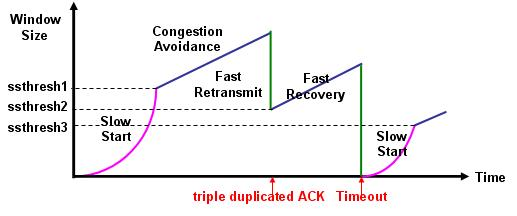
\includegraphics[scale = 0.55]{images/ssthreshold.jpg} 
    \caption{AIMD and SSThreshold}
    \label{aimd-ssthreshold}
\end{figure}
\subsection{Legacy TCP Versions}
Here there are a description of some TCP versions.
\subsubsection{TCP Tahoe}
Characteristics:
\begin{itemize}
    \item it has all TCP features previously described
    \item congestion control with AIMD + slow start + timeouts only for losses detection
\end{itemize}
\subsubsection{TCP Reno}
Characteristics:
\begin{itemize}
    \item it has both timeouts and 3 dupacks
    \item 3 dupacks is used to quickly recover from light congestion (1 packet loss)\\
    $\rightarrow$ without having a timeout
\end{itemize}
\subsubsection{TCP New Reno}
Characteristics:
\begin{itemize}
    \item it is like TCP Reno
    \item it introduces partial ACKs to recover more packets $\rightarrow$ without using timeouts\\
    $\rightarrow$ one recovery every RTT
\end{itemize}
\subsubsection{TCP SACK}
Characteristics:
\begin{itemize}
    \item it is the achronym for Selective ACK
    \item returning acks declares which packets were received
    \item all non received packets (no ACK) can be retransmitted\\
    $\rightarrow$ recover from multiple losses in just one RTT
\end{itemize}
\subsubsection{TCP Vegas}
\label{TCP-vegas-subsubsection}
Characteristics:
\begin{itemize}
    \item it is based on the assumption on throughput $\rightarrow$ actual $\leq$ expected\\
    where:
    \begin{itemize}
        \item[$\rightarrow$] actual = acks/round trip time
        \item[$\rightarrow$] expected = window size/round trip time
    \end{itemize} 
    \item reaction happens per congestion episode not per loss
    \item it includes some modification from basic TCP:
    \begin{itemize}
        \item[$\rightarrow$] modified Congestion Avoidance
        \item[$\rightarrow$] aggressive Retransmission
        \item[$\rightarrow$] aggressive Window Adaptation
        \item[$\rightarrow$] modified Slow-Start
    \end{itemize}
    \item \hypertarget{congestion-avoidance-paragraph}{Modified Congestion Avoidance}:
    \begin{itemize}
        \item[$\rightarrow$] throughput $\rightarrow$ actual $\leq$ expected
        \item[$\rightarrow$] expected throughput $\rightarrow$ it is transmission rate with no other traffic/queue
        \item[$\rightarrow$] Monitor transmission rate (throughput, goodput):
        \begin{itemize}
            \item Given static parameters $\alpha$,$\beta$ as values representing how many\\packets TCP Vegas can have in queues
            ($\alpha = 3$,$\beta = 1$)\\[0.15cm]
            $\rightarrow$ if $\alpha < \beta$
                $\Rightarrow$ expected $-$ $\beta <$ expected $-$ $\alpha <$ expected\\[0.15cm]
                $\rightarrow$ there are different scenarios:
            \begin{itemize}
                \item if expected $-$ $\alpha <$ actual $<$ expected\\
                $\Rightarrow$ decrease queues $\rightarrow$ increase rate\\
                $\Rightarrow$ low congestion $\rightarrow$ closer to expected
                \item if expected $-$ $\beta <$ actual $<$ expected $-$ $\alpha$\\
                $\Rightarrow$ don't do anything\\
                $\Rightarrow$ maybe congestion
                \item if actual $<$ expected $-$ $\beta$\\
                $\Rightarrow$ increase queues $\rightarrow$ decrease rate before packet drop\\
                $\Rightarrow$ high congestion $\rightarrow$ prevent packet loss
            \end{itemize}
        \end{itemize}
        \item[$\rightarrow$] CWND is updated every RTT $\rightarrow$ if:
        \begin{itemize}
            \item expected $-$ actual $< \alpha$\\
            $\Rightarrow$ CWND $=$ $\frac{\text{CWND} + 1}{\text{CWND}}$
            \item expected $-$ actual $> \beta$\\
            $\Rightarrow$ CWND $=$ $\frac{\text{CWND} - 1}{\text{CWND}}$
            \item $\alpha <$ expected $-$ actual $< \beta$\\
            $\Rightarrow$ CWND $=$ CWND
        \end{itemize}
        \begin{figure}[!h] 
            \centering 
            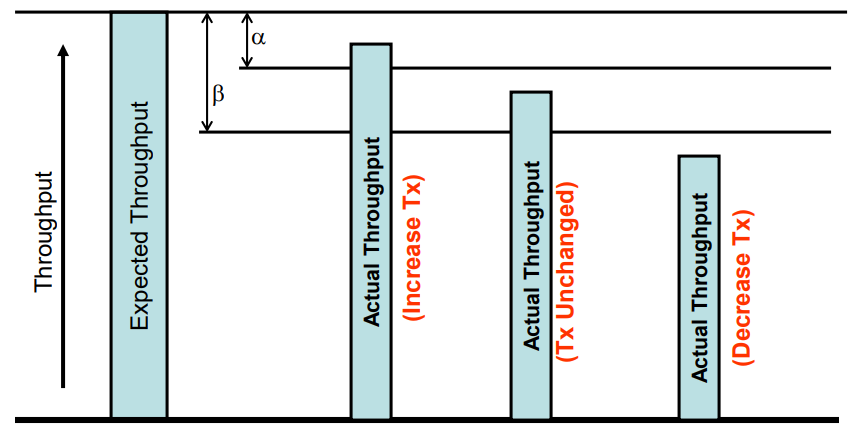
\includegraphics[scale = 0.35]{images/congestion-avoidance-vegas.png} 
            \caption{Modified Congestion Avoidance in TCP Vegas}
            \label{congestion-avoidance-vegas}
        \end{figure}
    \end{itemize}
    \item Aggressive Retransmission $\rightarrow$ with 3 dupacks:
    \begin{itemize}
        \item[$\rightarrow$] 1\textsuperscript{st} and 2\textsuperscript{nd} packets $\rightarrow$ it checks timeout
        \item[$\rightarrow$] if timeout expires $\Rightarrow$ immediately retransmission
    \end{itemize}
    \item Aggressive CWND update $\rightarrow$ 3 different types of update:
    \begin{itemize}
        \item[$\rightarrow$] recovery $\rightarrow$ CWND becomes $\frac{3}{4}$ when it enters into recovery\\
        $\rightarrow$ instead of $\frac{1}{2}$
        \item[$\rightarrow$] multiple loss $\rightarrow$ CWND is reduced by 1 size
        \item[$\rightarrow$] initial setting $\rightarrow$ CWND is set on dimension 2 $\rightarrow$ instead of 1 
    \end{itemize}
    \item Modified Slow Start:
    \begin{itemize}
        \item[$\rightarrow$] TCP keeps the congestion window fixed in every
        other RTT\\$\rightarrow$ it measures the throughput
        \item[$\rightarrow$] Given:
        \begin{itemize}
            \item static parameter $\gamma$ as value $\frac{1 \text{packet}}{RTT}$
            \item actual and expected throughput defined as backwards (§\ref{TCP-vegas-subsubsection})
        \end{itemize}
        on every next RTT, it does the followings:
        \begin{itemize}
            \item if expected $-$ actual$< \gamma$ $\rightarrow$ continue Slow Start:
            \begin{itemize}
                \item CWND $=$ $2$ $\cdot$ CWND for each RTT
                \item CWND = CWND $+$ $1$ for each ACK
                \item[$\Rightarrow$] Exponential Increase
            \end{itemize}
            \item if expected $-$ actual$> \gamma$ $\rightarrow$ switch to Congestion Avoidance:
            \begin{itemize}
                \item Set SSThreshold $=$ CWND
                \item follow \hyperlink{congestion-avoidance-paragraph}{Congestion Avoidance}'s rules written before
            \end{itemize}
            \begin{figure}[!h] 
                \centering 
                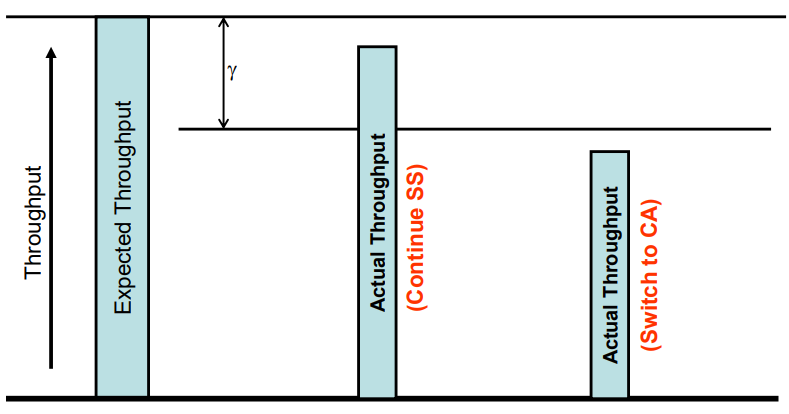
\includegraphics[scale = 0.4]{images/slow-start-vegas.png} 
                \caption{Modified Slow Start in TCP Vegas}
                \label{modified-slow-start-vegas}
            \end{figure}
        \end{itemize}
    \end{itemize}
    \item Retrocompatibility:
    \begin{itemize}
        \item[$\rightarrow$] it is sensible to delay variations
        \item[$\rightarrow$] it can't coexists with other versions
        \item[$\rightarrow$] Example:\\[0.15cm]
        When a TCP Vegas flow shares the same bottleneck with a TCP New Reno\\
        $\rightarrow$ as soon as the pipe is full and packets get buffered\\
        $\Rightarrow$ TCP Vegas reduces its data rate\\
        $\Rightarrow$ more space to TCP New Reno\\
        $\rightarrow$ it continues its growth till congestion
    \end{itemize}
    \item[$\rightarrow$] for the example this makes vegas not used $\rightarrow$ but it inspires other protocols
\end{itemize}